\subsection{Módulo MP3}
El modelo de MP3 seleccionado ha sido el YX5300, el cual se muestra en la \autoref{fig:2-3-MP3}.

Este reproductor se comunica con el microcontrolador mediante UART. También cuenta con una frecuencia de muestreo de 48 kHz y soporta tanto el formato MP3 como el formato WAV. Este modelo cuenta con un socket de tarjeta microSD en la cual se introducen las canciones, en los formatos antes mencionados, que se deseen reproducir.

\begin{figure}[h]
    \centering
    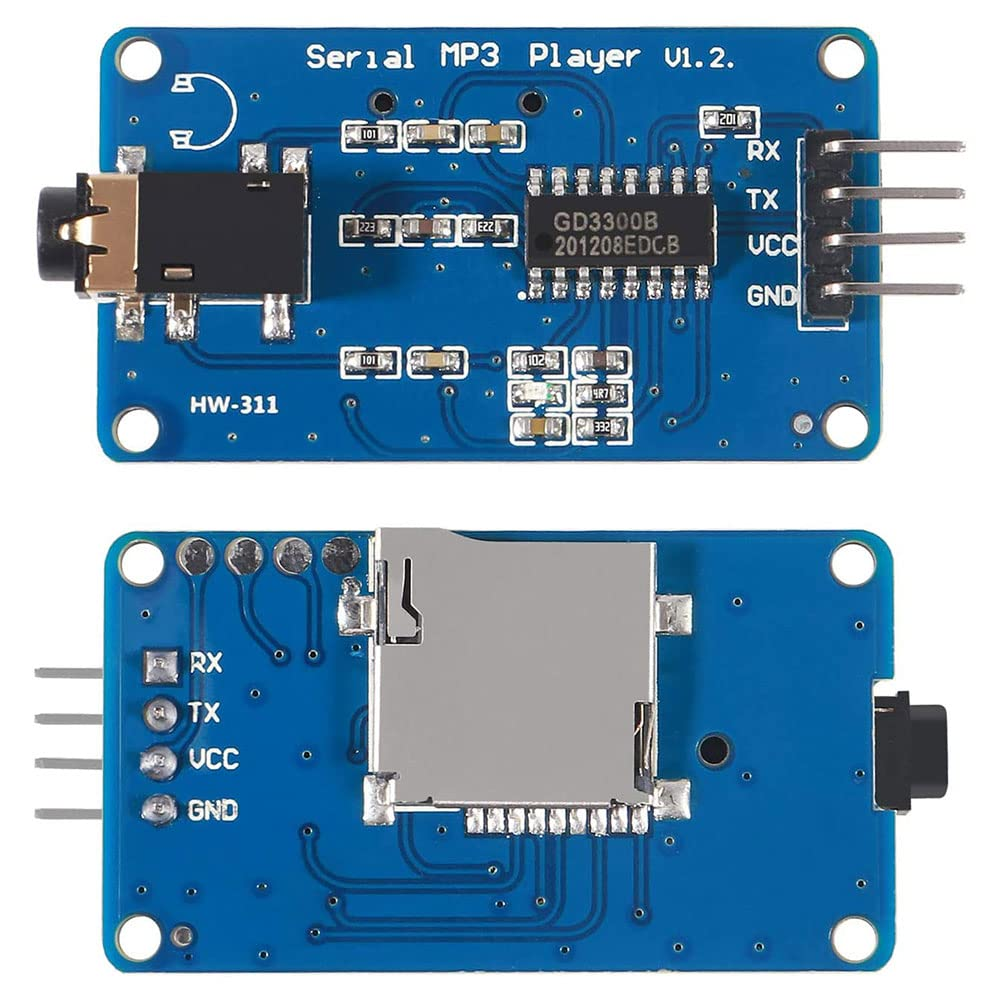
\includegraphics[width=0.3\textwidth]{images/2/2-4/MP3.jpg}
    \caption{Reproductor MP3 YX5300}
    \label{fig:2-3-MP3}
\end{figure}